\section{Background}
In this section we give the necessary background for the buddy allocation algorithms we provide the specification for, and the Isabelle/HOL theorem prover that we use for its specification and verification.

\subsection{Buddy Allocation Algorithm}
Generally, the buddy algorithms~\cite{reg_knowlton} in which each block is subdivided into two smaller blocks are the simplest and most common variety. The main idea is that when a larger block is split, it is divided into two smaller blocks, and each smaller block becomes an unique buddy to the other. A split block can only be merged with its unique buddy block, which then reforms the larger block they were split from. With this way, buddy memory system has small external fragmentation when compared with other dynamic allocation techniques.

To implement buddy allocation algorithms, it applies two important data structures multilevel free linked-list and multilevel free bitmap. The first one is used to manage free blocks at each level. The block to be allocated or deallocated is directly picked from the head of linked-list or added into the tail. Bitmap is used to quickly check if blocks belonging to the same parent are free, in order to decide whether to merge these blocks into one block. Fig. \ref{fig3} describes a moment in memory system using these two date structures.

\begin{figure}
	\centering
	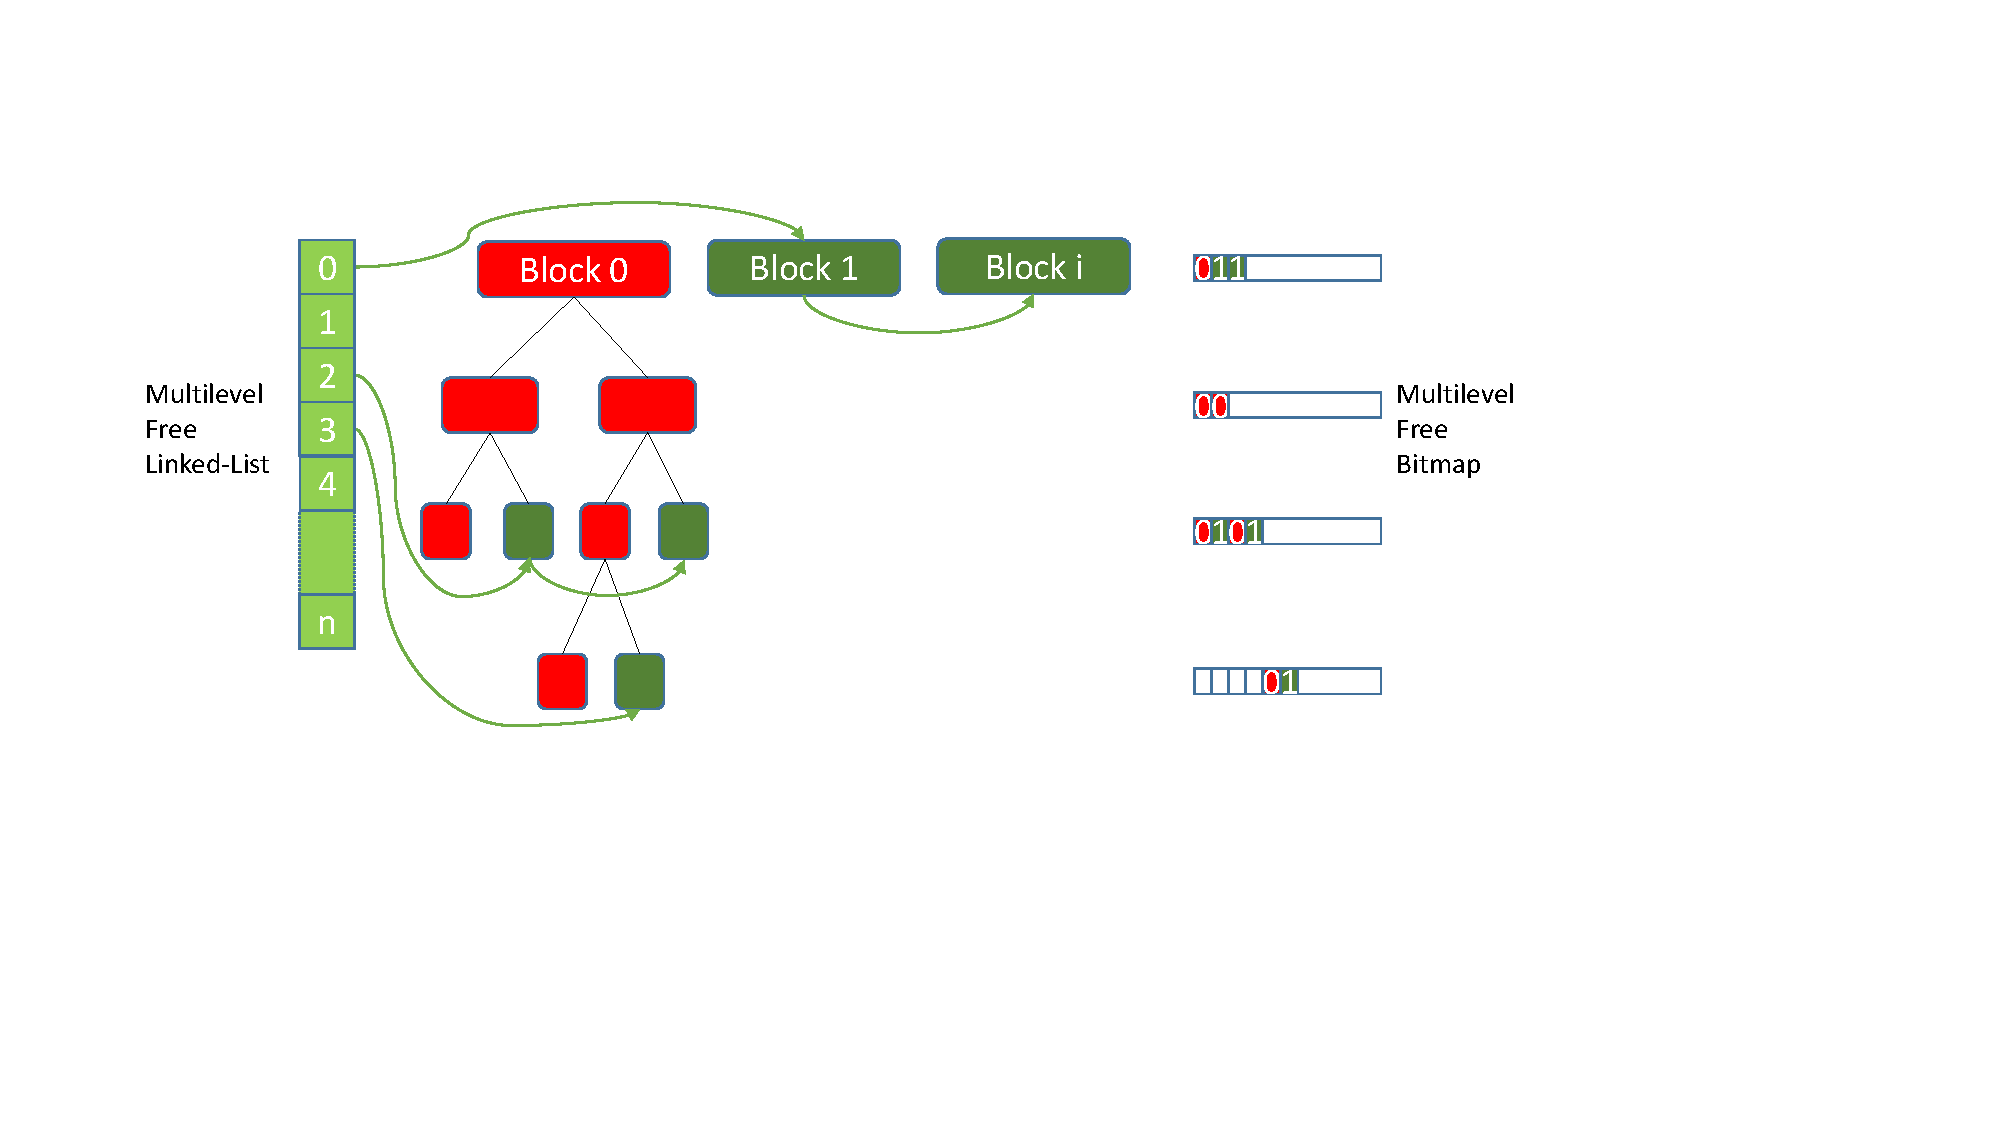
\includegraphics[width=1\textwidth]{fig3.pdf}
	\caption{Structures in Buddy Allocation Algorithms}
	\label{fig3}
\end{figure}

\subsection{Isabelle/HOL}
We use the interactive theorem prover Isabelle/HOL~\cite{reg_Isabelle/HOL} to conduct the specification and verification of the memory management. Isabelle/HOL is a higher order logic theorem prover, using a typed lambda calculus-like functional language for specifications. 

Isabelle/HOL includes a specification for simple common types such as naturals, integers, and booleans. It also specify some composed data types like tuples, records, lists, and sets that are parametrized on other types. Isabelle provides the interface \emph{datatype} for the creation of user defined types based on type constructors. 

Isabelle provides functions on predefined types to access their members or to provide additional operations over them. In the following we describe those functions that we use along this work. Tuples are denoted as (\emph{$t_1$} $\times$ \emph{$t_2$}), projection function \emph{fst} and \emph{snd} respectively returns elements $t_1$ and $t_2$. Lists are defined as a datatype with an empty construct denoted with \emph{NIL} or $[]$, and a concatenation construct denoted with $\#$, where $x\#xs$ adds $x$ to the front of $xs$. The $i$th component of a list $as$ is written as $as!i$. Isabelle/HOL provides functions for definite and indefinite descriptions. Definitive descriptions are represented by $THE\ x.\ P\ x$ and return the element uniquely described by the predicate $P$, else it returns and undefined value. Indefinite descriptions are represented by $SOME\ x.\, P\ x$ selecting a random element from the predicate $P$ that must describe at least one element, else it returns an arbitrary value.

Isabelle/HOL allows user to create non-recursive specifications using the command \textbf{definition}, and to create recursive specifications using commands \textbf{primrec} and \textbf{recursive}.

%The notation {\isasymlbrakk} $A_1$;\dots;$A_n${\isasymrbrakk} $\Longrightarrow$ A represents an implication with assumptions $A_1$;\dots;$A_n$ and conclusion A. Isabelle mainly employs backward deduction, which means to prove the main goal, we must firstly prove subgoals which are decomposed from the main goal. It uses the rules of the reasoning like introduction, elimination, destruction rules, etc., as well as automatic provers such as \emph{SMT}.
